\chapter{Fibonacci Sequence}

%~ \vskip -15pt

%~ \centerline{{\LARGE\sl Understanding IP Routing}}


\vskip 0.8cm

\begin{center}
{\large\uppercase{$\text{Arulalan Rajan, R. Vittal Rao, H. S. Jamadagni}$}} 

\vskip -6pt

Department of Electronic Systems Engineering,\\ Indian Institute of Science,\\ Bengaluru - 560012, India 

\end{center}


\begin{center}
{\large\uppercase{$\text{Ashok Rao}$}} 

\vskip -6pt

Consultant, 165, 11th main,\\ Saraswathipuram,\\ Mysore, India

\end{center}



\vfill




\newpage

\begin{multicols}{2}

Fibonacci sequence, among the ocean of integer sequences, has caught the attention of professional mathematicians and amateurs alike, for over centuries. While on the one side, it is a treasure house of numerous interesting mathematical properties, on the other side, the applications of Fibonacci sequence are widespread, including that of fractal music, financial market trading etc. Fibonacci numbers are found in many biological settings and nature, like the number of petals in sunflower, spiral phyllotaxis of plants and so on.

The elements of the Fibonacci sequence are generated by the second order recurrence relation
$$
f_{n}=f_{n-1}+f_{n-2}
$$
, with the condition that $f_{0} = 0, f_{1} = 1$. It is also interesting to note that for a number $x$. to be a Fibonacci number, either $5x^{2} + 4$ or $5x^{2}-4$ must be a a perfect square.

The ratio
$$
{\rm \lim_{{\it n} \rightarrow \infty}} \dfrac{f_{n}+1}{f_{n}}
$$

converges to the golden mean or the golden ratio\break $\varphi =\dfrac{1+\sqrt{5}}{2}$

The n-th Fibonacci number can be expressed in terms of the golden ratio as

$$
f_{n}= \dfrac{\varphi-(-\varphi^{-}n}{\sqrt{5}}
$$

In this work, we unfold yet another interesting result related to Fibonacci sequence from the perspective of discrete probability distributions generated by linear recurrence relations.\raisebox{-.1cm}{\includegraphics[scale=.9]{src/Figures/circledC.eps}}


\end{multicols}


